% ======================================================================
\section{Linear subspace methods}
\label{sec:linear}
% ======================================================================

\subsection{Proper orthogonal decomposition}
\label{sec:pod}

Proper orthogonal decomposition (POD), known in statistics as principal
component analysis (PCA) \parencite{pearson1901,hotelling1933} and in stochastic
processes as the Karhunen--Lo\`eve expansion, was introduced to turbulence by
\textcite{lumley1967} as an objective definition of coherent structures. Given
the snapshot matrix \eqref{eq:snapshots}, POD seeks the orthonormal basis
$\{\bm{\phi}_j\}_{j=1}^{r}$ that maximizes the average projected energy or,
equivalently, minimizes the mean-square reconstruction error
\begin{equation}
  \min_{\Phib^{\top}\W\Phib=\bm{I}}\;\sum_{k=1}^{T}\bigl\|\bm{x}_k-\Phib\Phib^{\top}\W\bm{x}_k\bigr\|_{\W}^{2},
  \label{eq:pod}
\end{equation}
whose solution is given by the leading left singular vectors of
$\W^{1/2}\X$. With the singular value decomposition
$\W^{1/2}\X=\bm{U}\bm{\Sigma}\bm{V}^{\top}$, the modes are
$\Phib=\W^{-1/2}\bm{U}_{:,1:r}$, the temporal coefficients are
$\z_k=\Phib^{\top}\W\bm{x}_k$, and the eigenvalues $\lambda_j=\sigma_j^2$ are the
energies of the modes. By the Eckart--Young theorem \parencite{eckart1936},
the truncation error is $\sum_{j>r}\lambda_j$, so no rank-$r$ linear
representation of the \emph{training} data is more accurate in this norm. When
$T\ll N$, as is typical for simulation data, the \emph{method of snapshots}
\parencite{sirovich1987} obtains the same modes from the $T\times T$
correlation matrix $\X^{\top}\W\X$. The theory and early applications to wall
turbulence and transitional flows are reviewed by \textcite{berkooz1993} and
\textcite{holmes2012turbulence}.

POD has several properties that explain its dominance as the first stage of
fluid-dynamics ML pipelines. Its encoder and decoder are linear, cheap, and
exactly inverse on the subspace. The modes are orthogonal and ranked by
energy. For many flows the leading modes have clear physical meaning, for
example the pairs of traveling-wave modes associated with vortex shedding. The
construction requires no hyperparameters beyond $r$. Scalable algorithms are
mature: randomized SVD \parencite{halko2011} and incremental or streaming SVD
\parencite{levy2000,brand2006} make POD feasible for data sets that do not fit
in memory.

\Cref{fig:ldc_pod} shows POD applied to a two-dimensional lid-driven cavity at
$\mathrm{Re}=15{,}000$, the dataset used for the computed examples in this
review. The leading modes are organized along the shear layers and walls of the
cavity. The first two modes form a traveling-wave pair that together capture
about 90\% of the fluctuation energy, and eight modes capture 99\%. A spectrum
this steep indicates a flow dominated by a small number of coherent
oscillations, the regime in which global POD is most effective. We return to
this point when comparing global and local bases in \cref{sec:dls}.

\begin{figure}[tbp]
  \centering
  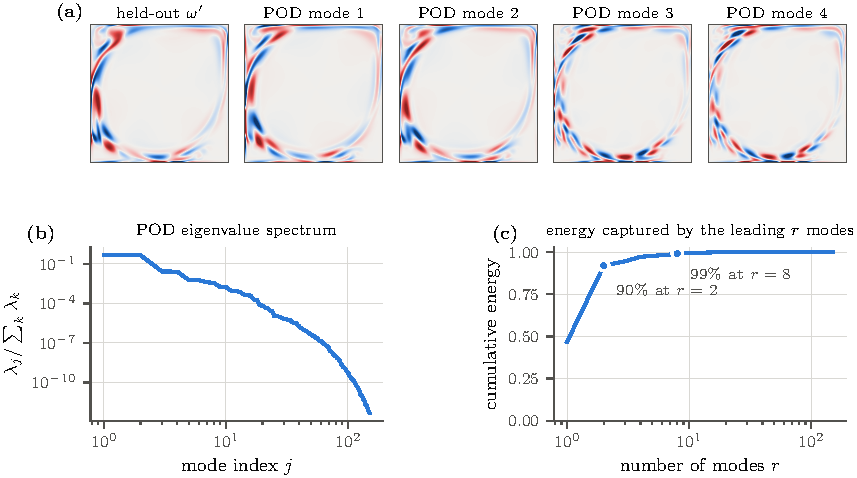
\includegraphics[width=\textwidth]{figs/ldc_pod.pdf}
  \caption{POD of the two-dimensional lid-driven cavity at $\mathrm{Re}=15{,}000$
  (2000 training snapshots, weighted $L^2$ inner product). (a)~Fluctuating
  vorticity of a held-out snapshot and of the four leading POD modes;
  (b)~normalized eigenvalue spectrum (modes with $\lambda_j>10^{-12}\lambda_1$);
  (c)~cumulative energy fraction, with the number of modes needed to capture
  90\% and 99\% of the fluctuation energy.}
  \label{fig:ldc_pod}
\end{figure}

\paragraph{POD in intrusive models.}
The classical use of POD is Galerkin projection of the Navier--Stokes equations
onto the leading modes. Early landmarks include the low-dimensional model of
the turbulent wall layer of \textcite{aubry1988}, and the hierarchy of cylinder
wake models of \textcite{noack2003hierarchy}, which introduced a ``shift mode''
to represent the mean-flow deformation that POD modes of the limit cycle
miss. Two difficulties of POD--Galerkin models motivate much of the later
data-driven work. First, truncation removes the small scales that dissipate
energy, so truncated models are often unstable or inaccurate without closure
\parencite{wang2012closure,ahmed2021closures}. Second, evaluating the nonlinear
term still scales with $N$ unless hyper-reduction is used, for example the
empirical and discrete empirical interpolation methods
\parencite{barrault2004eim,chaturantabut2010deim} or GNAT with least-squares
Petrov--Galerkin (LSPG) projection
\parencite{carlberg2011lspg,carlberg2013gnat,carlberg2017galerkin}.

\paragraph{POD in non-intrusive, learned models.}
Because POD coefficients form a compact, ordered, and decorrelated set of
features, they are the most common input to learned surrogate models. In
parametric problems, regression maps from parameters (and time) to POD
coefficients have been built with neural networks
\parencite{hesthaven2018podnn} and Gaussian processes \parencite{guo2019gpr}.
PCA-Net extends the idea to operator learning by applying PCA to both input and
output function spaces \parencite{bhattacharya2021pcanet}. For time-series
prediction, POD coefficients have been advanced by extreme learning machines
used as closures \parencite{san2018elm} and by recurrent networks:
long short-term memory (LSTM) models of POD coefficients were proposed by
\textcite{wang2018model} and by \textcite{mohan2018lstm} for turbulent-flow
control, deep feedforward networks with residual and backward-difference update
formulas by \textcite{pawar2019deep}, and LSTMs and neural ordinary differential
equations, including closure of unresolved modes, by
\textcite{maulik2020timeseries}. More recently, transformers have been applied
to POD coefficients of flows past a cylinder and a group of buildings
\parencite{wu2022transformer}. Operator inference fits polynomial reduced
operators directly to projected trajectories
\parencite{peherstorfer2016opinf,qian2020liftlearn,kramer2024opinf}; it is
non-intrusive but, unlike black-box regression, retains the structure of a
projection-based ROM. \textcite{swischuk2019projection} compare several such
POD-plus-regression formulations and argue that the projection structure is
itself a useful physics-based inductive bias.

\subsection{Dynamics- and frequency-aware decompositions}
\label{sec:dmd}

POD ranks modes by energy but ignores temporal order. Several decompositions
incorporate dynamics or frequency content and are frequently used either as
the reduced representation or as a diagnostic of it.

\emph{Dynamic mode decomposition} (DMD) fits a best linear operator
$\bm{A}$ with $\bm{x}_{k+1}\approx\bm{A}\bm{x}_k$ and represents the data by
its eigenvectors, each oscillating at a single frequency with a single growth
rate \parencite{schmid2010dmd}. \textcite{rowley2009spectral} interpreted DMD
as a finite-dimensional approximation of the Koopman operator
\parencite{mezic2005,mezic2013}. Exact DMD \parencite{tu2014dmd}, extended DMD
with nonlinear dictionaries \parencite{williams2015edmd}, sparsity-promoting DMD
\parencite{jovanovic2014spdmd}, and optimized DMD \parencite{askham2018optdmd}
are variants that improve robustness or mode selection; see
\textcite{kutz2016dmd} and \textcite{brunton2022koopman} for reviews. For
learning, the appeal of DMD and Koopman methods is that they provide
coordinates in which the dynamics are (approximately) linear, an idea that
reappears in Koopman autoencoders (\cref{sec:koopman}).

\emph{Spectral POD} (SPOD) computes POD modes of each temporal frequency from
the cross-spectral density, yielding modes that are coherent in both space and
time and optimal for statistically stationary flows
\parencite{towne2018spod,schmidt2020guide}. Towne et al.\ showed that SPOD modes
coincide with DMD modes and with resolvent modes
\parencite{mckeon2010critical} under particular assumptions. A distinct method
with the same name filters the POD correlation matrix along its diagonals to
interpolate between POD and a Fourier decomposition \parencite{sieber2016spod}.
\emph{Multi-scale POD} (mPOD) combines a filter bank with POD so that each
mode is confined to a frequency band \parencite{mendez2019mpod}, which is
relevant for flows with several separated time scales.
\emph{Balanced POD} \parencite{rowley2005bpod} approximates balanced truncation
\parencite{moore1981} using snapshots of the direct and adjoint systems, and
selects modes by input--output importance rather than energy. This matters
for control-oriented models, where low-energy structures can dominate the
response.

\subsection{Limits of global linear reduction}
\label{sec:barrier}

The optimality of POD is optimality \emph{among linear subspaces for the
training data}. Two limitations follow.

\paragraph{The transport barrier.}
When coherent features move, such as a vortex advected through the domain, a
shock translating with a parameter, or a flame front, the set of states is a
low-dimensional but strongly curved manifold whose linear span is large. For
the linear advection equation with discontinuous data, the Kolmogorov $n$-width
\eqref{eq:nwidth} decays only as $r^{-1/2}$
\parencite{ohlberger2016reduced,greif2019decay}. \Cref{fig:nwidth} shows the
effect on the singular values of simple one-dimensional snapshot sets. For a
diffusing Gaussian pulse the singular values fall below $10^{-10}$ within
about twenty modes. For the same pulse advected across the domain they decay
far more slowly. For an advected discontinuity they remain above $10^{-2}$ for
more than a hundred modes, until the snapshot matrix runs out of rank. Such
problems are common in fluid dynamics: shear layers, wakes, jets, cavity
flows with convecting vortices, and shocks all feature transport.

Within the linear framework, the barrier can be mitigated by transforming the
data before POD so that the features no longer move. Approaches include
symmetry reduction and template fitting \parencite{rowley2000symmetry},
Lagrangian or characteristic-based bases \parencite{mojgani2017lagrangian},
shifted POD with multiple transport velocities \parencite{reiss2018spod},
optimal-transport advection modes \parencite{iollo2014advection},
transport reversal \parencite{rim2018transport}, transported snapshots
\parencite{nair2019transported}, and learned registration maps
\parencite{taddei2020registration,mojgani2021registration}. All of these build
a \emph{nonlinear} trial manifold out of a linear basis and a nonlinear
transformation, and they anticipate the neural approaches of
\cref{sec:autoencoders}. \textcite{peherstorfer2022breaking} provides a concise
review of this line of work.

\paragraph{Multi-scale content and generalization.}
High-Reynolds-number turbulence poses a related difficulty even without a
dominant transport direction. The energy spectrum is broadband, so the POD
eigenvalues decay slowly and the small scales, which carry a small share of the
energy but most of the dissipation and much of the intermittency, sit at the
end of the spectrum. The global modes also have global support: a mode that
represents a structure in one region must also be ``paid for'' everywhere
else. In addition, the rank of a snapshot POD basis cannot exceed the number
of training snapshots, so for flows with many active scales the amount of
training data needed grows with the desired accuracy. It is well documented
that POD bases can be inefficient for multi-scale turbulent flows
\parencite{berkooz1993,deshmukh2016sparse,deshmukh2020dls}. Parametric variation
adds a third difficulty: a basis built at one operating condition may not
represent another. Common remedies are interpolation of bases on the
Grassmann manifold \parencite{amsallem2008grassmann} and the local and
clustered bases discussed next.

\begin{figure}[tbp]
  \centering
  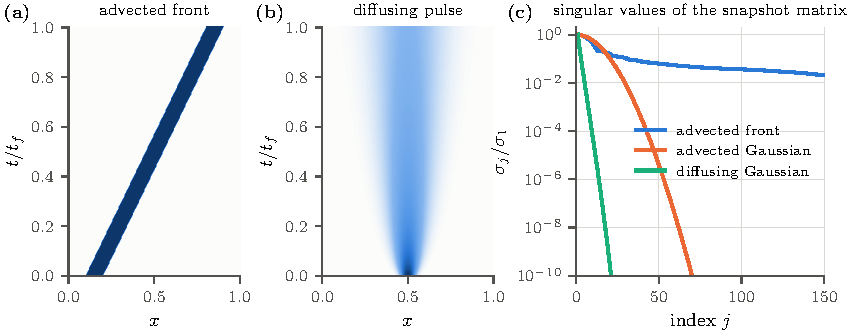
\includegraphics[width=\textwidth]{figs/nwidth.pdf}
  \caption{The transport barrier for linear reduction. (a)~An advected
  discontinuity (top-hat of width 0.1) and (b)~a diffusing Gaussian pulse,
  shown in space--time. (c)~Normalized singular values of the corresponding
  snapshot matrices (200 snapshots, 256 grid points), together with an
  advected Gaussian of the same width as the diffusing pulse. All three
  data sets are one-parameter families, yet for a given accuracy the advected
  families need several times (Gaussian) to tens of times (discontinuity) more
  linear modes than the diffusing one.}
  \label{fig:nwidth}
\end{figure}
